\section{How to include figures}\label{sec6}

\subsection{Figures}

Figures must be inserted directly into the main text of the manuscript and should not be placed collectively at the end. All figures must be cited in the main text in numerical order, and each figure should be placed immediately after the paragraph in which it is first mentioned.

All figures must be presented in a size and format that ensure clear readability. Each figure must be accompanied by an appropriate caption or legend. Figures should be numbered consecutively throughout the manuscript using Arabic numerals (for example, Figure 1, Figure 2, and Figure 3). For figures appearing in an appendix, the numbering should be prefixed with the appendix letter (for example, Figure A1 and Figure B1).

Authors are strongly encouraged to use two-dimensional (2D) graphics rather than three-dimensional (3D) graphics unless a 3D representation is essential, as 2D graphics are generally clearer, more accurate, and easier to interpret. Border lines around figures should be removed. Authors should also avoid the use of white text and background colors in figures, as these may reduce legibility.

When referring to figures in the manuscript text and in figure captions, authors must use the full term “Figure” rather than the abbreviation “Fig.”

Note that your figure will automatically be placed in the most appropriate place for it, given the surrounding text and taking into account other figures or tables that may be close by. You can find out more about adding images to your documents in this help article on \href{https://www.overleaf.com/learn/how-to/Including_images_on_Overleaf}{including images on Overleaf}.



\begin{figure}[!ht]
\centering

\includegraphics[width=0.5\linewidth]{z_cat_momo_1.png}
\caption{\label{fig:cat1}This cat picture is located at the 'figures' folder.}
\end{figure}


If a figure consists of multiple subfigures as shown in Figure 2, each subfigure should be identified by a capital letter, such as (A), (B), (C), and so forth, centered below the corresponding subfigure. Authors should follow the style illustrated in Figure 2 of the manuscript template. Subfigure labels must not be embedded within the image itself.

When citing a figure that contains multiple subfigures in the main text, authors should use the format Figure 2A, Figure 2B, and so on. In the figure caption, the corresponding descriptions should be given using the format (A), (B), (C), etc.

When multiple images are combined into a single figure using a grid arrangement, authors should ensure that the layout does not compromise visibility. In particular, placing too many images in a single horizontal row may reduce the size of each image and make textual or graphical details difficult to read. Where necessary, authors should reduce the number of images arranged horizontally. For example, if a 2 × 4 layout results in images that are too small, a 4 × 2 layout may provide better visibility.


\begin{figure}[!ht]
    \centering
    \begin{subfigure}{0.45\textwidth}
        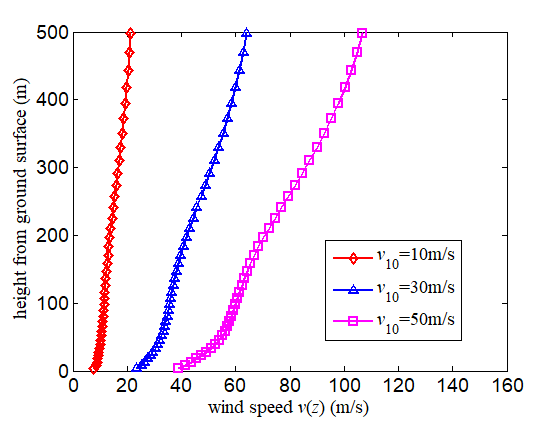
\includegraphics[width=\linewidth]{z_fig_a.png}
        \caption{}
    \end{subfigure}
    \hfill
    \begin{subfigure}{0.45\textwidth}
        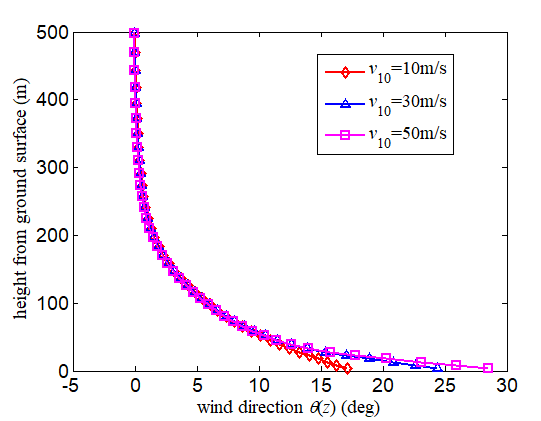
\includegraphics[width=\linewidth]{z_fig_b.png}
        \caption{}
    \end{subfigure}
    \vskip\baselineskip
    \begin{subfigure}{0.45\textwidth}
        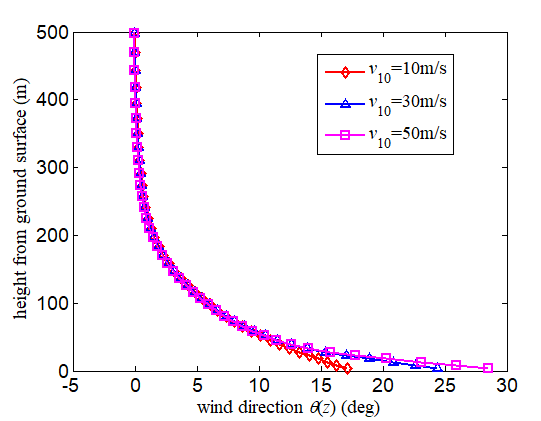
\includegraphics[width=\linewidth]{z_fig_c.png}
        \caption{}
    \end{subfigure}
    \hfill
    \begin{subfigure}{0.45\textwidth}
        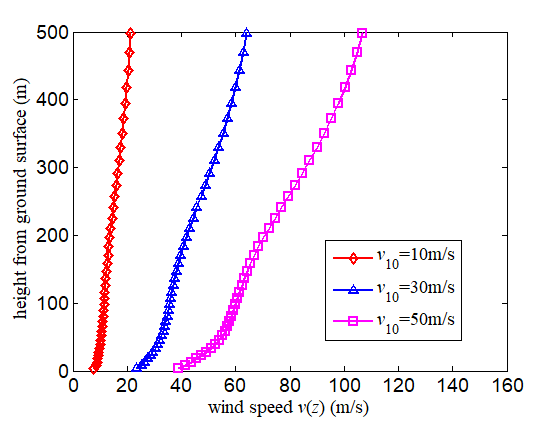
\includegraphics[width=\linewidth]{z_fig_a.png} % 첫 번째 그림 다시 사용
        \caption{}
    \end{subfigure}
    \caption{Overall caption for the four figures. (A) Caption for figure A. (B) Caption for figure B. (C) Caption for figure C. (D) Caption for figure D.}
    \label{fig:multi_figs}
\end{figure}

\subsection{Alt text}

Incorporating alt text (alternative text) when submitting your paper helps to foster inclusivity and accessibility. Well-written alt text enables readers with visual impairments, including those using screen readers, to understand the content and context of your figures. The purpose of alt text is to provide concise, informative descriptions of the essential information conveyed by each figure so that all readers have equitable access to the same information and can engage with the visual elements integral to scholarly content. Including alt text demonstrates a commitment to accessibility and can enhance the overall impact and reach of your work. Although some journals include alt text below each figure caption, as shown in Figure \ref{fig:alt_text}, for administrative convenience we ask authors to submit a separate MS Word file containing a list of all alt texts once the manuscript has been accepted.
Please note the following points regarding alt text:
\begin{itemize}
\item Alt text applies to all images, figures, illustrations, and photographs.
\item Alt text is primarily accessed via assistive technologies (e.g., screen readers) and may not appear in the typeset article.
\item Once the manuscript has been accepted, please submit alt text in a separate MS Word file.
\item \href{https://static.primary.prod.gcms.the-infra.com/static/site/journals/document/alt-text-figure-accessibility.pdf?node=1329505d4d63d87a12ed}{Detailed guidance on how to draft and submit alt text.}
\end{itemize}


\begin{figure}[!ht]
\centering
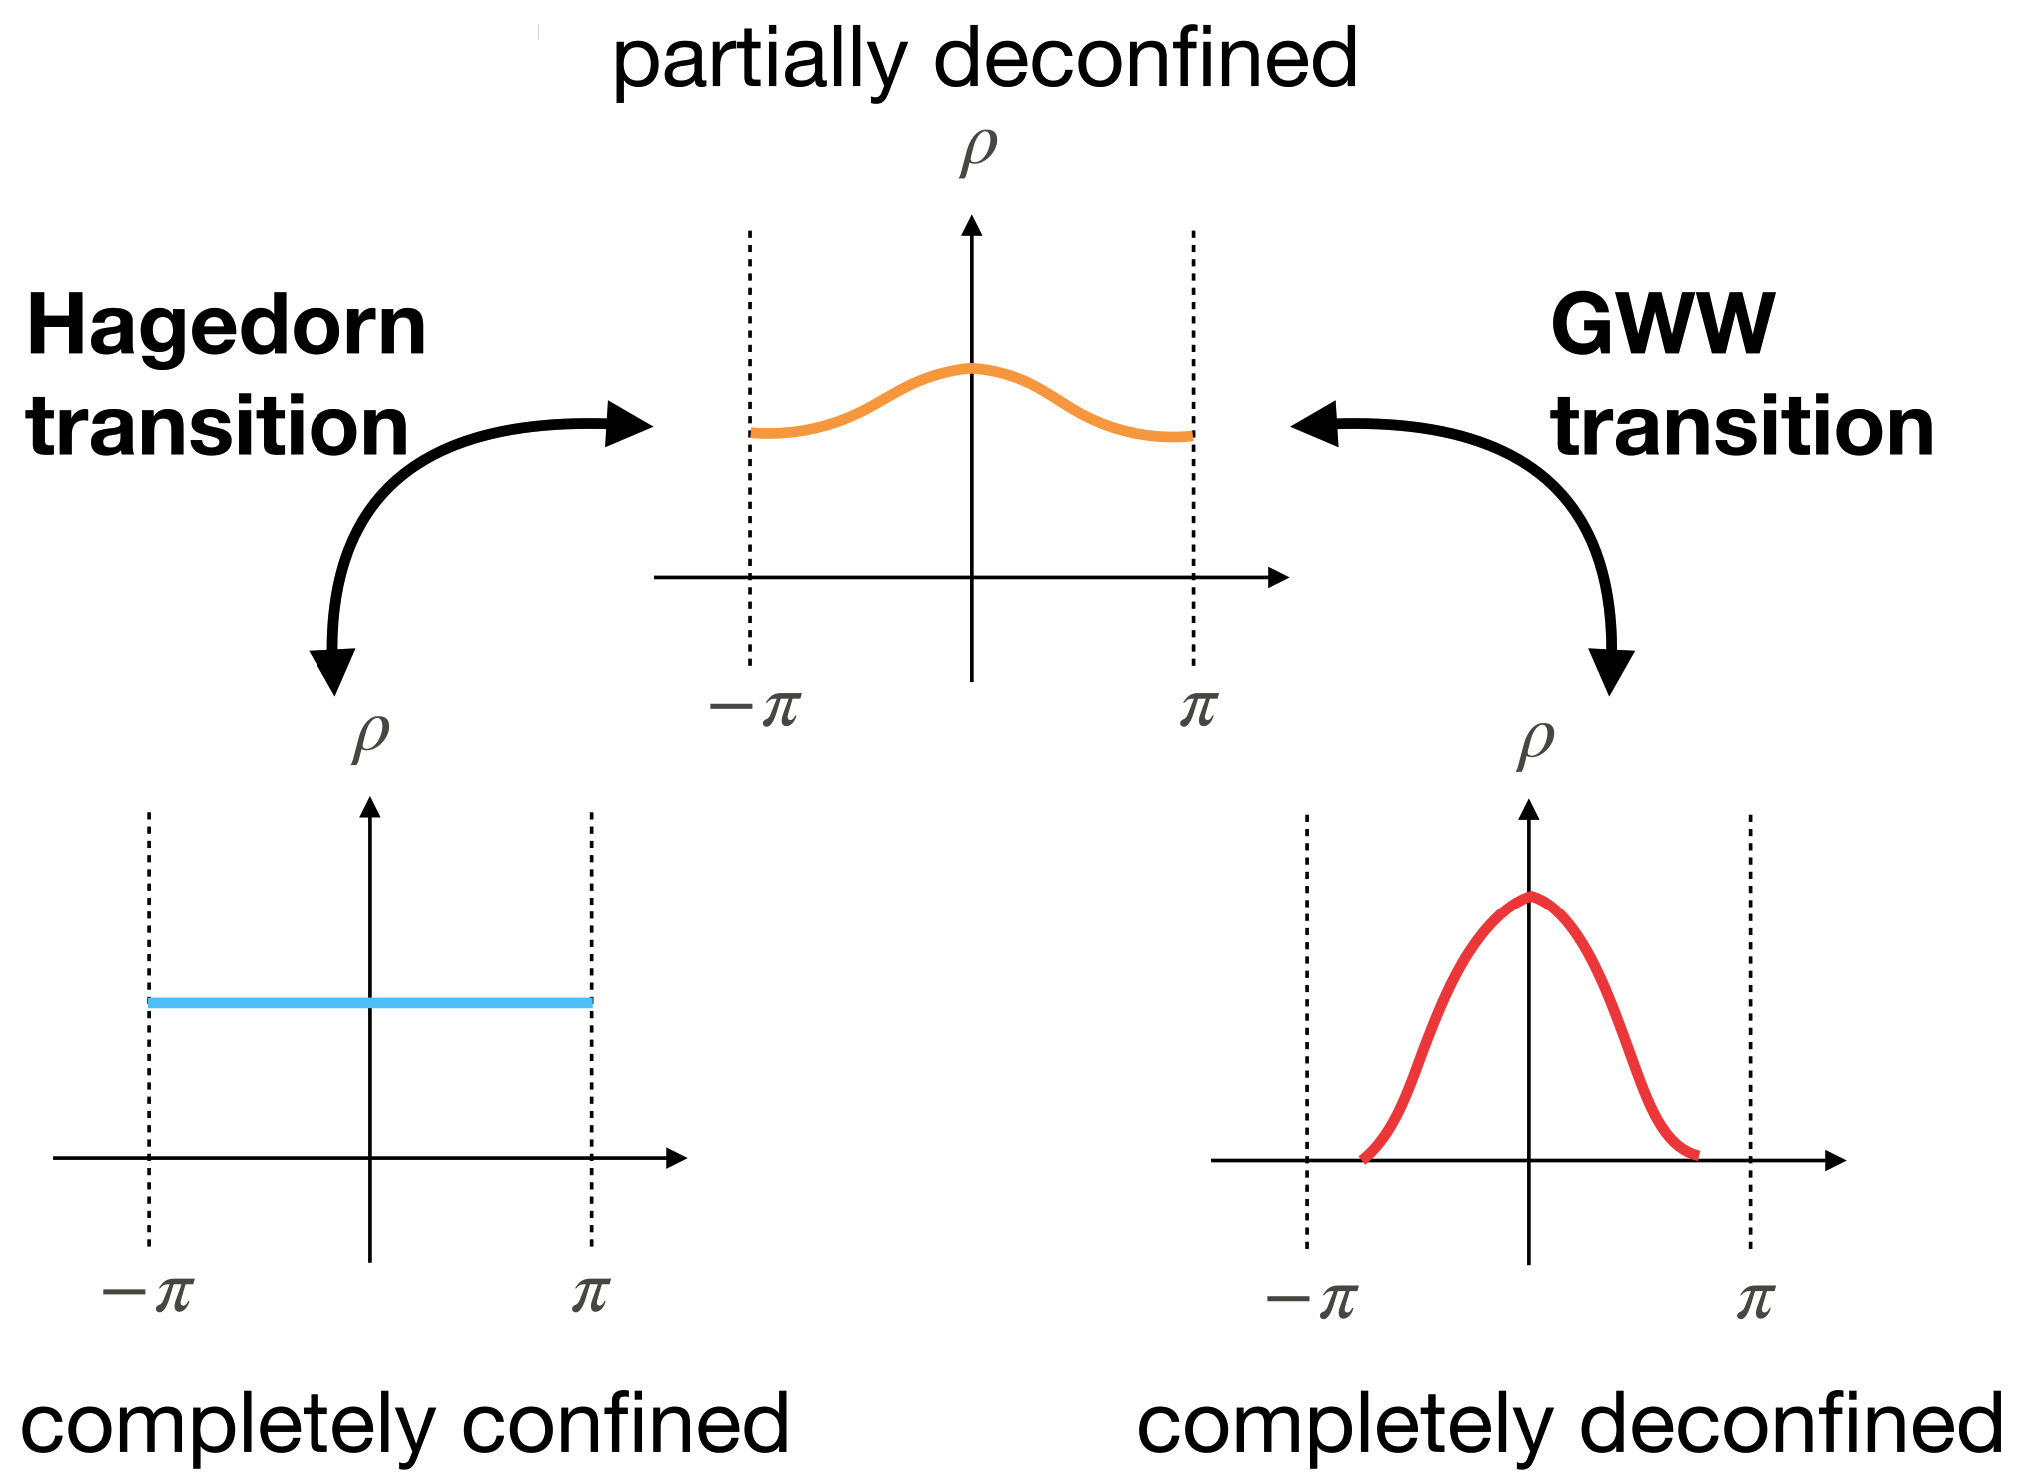
\includegraphics[width=0.7\linewidth]{z_alt_text_example.png}
\caption{\label{fig:alt_text}Completely confined, partially deconfined, and completely deconfined phases correspond to uniform, nonuniform but jointed, and disjointed distributions of Polyakov line phases, respectively.\\
\textbf{Alt Text:} Graphical representation of three phases—completely confined, partially deconfined, and completely deconfined—depicting Polyakov line phases with corresponding transition profiles.
}
\end{figure}

%--- Section ---%
